% ============================================================
% FIGURE: the boundary. Built 2026-07-27 from exp_AA CSVs, not from summaries.
%   panel (a)  exp_AA/results_armB.csv  metis + lspar, mu=0.5, all statuses
%              exp_AA/results_armA.csv  leiden + lspar, mu=0.5, status ok
%   panel (b)  exp_AA/results_armB.csv  metis + lspar, mu=0.5, all statuses
% Panel (a)'s Metis series and panel (b) are the mean dQ and mean dAMI columns of
% Table~\ref{tab:boundary} and must stay identical to it.
%
% Colours are Okabe-Ito #0072B2 and #D55E00, a published colour-vision-deficiency
% -safe pair. The palette validator could not be run in this environment, so the
% figure does not rely on hue alone: the series differ in dash pattern and marker
% shape and read correctly in greyscale.
% ============================================================
\begin{figure*}[t]
\centering
\definecolor{cbblue}{HTML}{0072B2}
\definecolor{cbvermillion}{HTML}{D55E00}
%
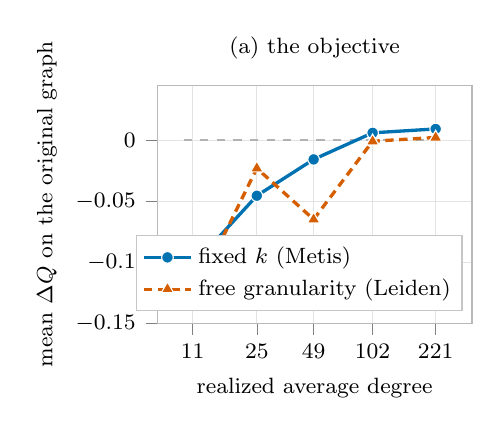
\begin{tikzpicture}
\begin{axis}[
    width=0.46\textwidth, height=4.6cm,
    xmode=log, log basis x=10,
    xlabel={realized average degree},
    ylabel={mean $\Delta Q$ on the original graph},
    xtick={11.2,24.6,49.4,101.9,220.9},
    xticklabels={11,25,49,102,221},
    xticklabel style={font=\footnotesize},
    scaled y ticks=false,
    yticklabel style={font=\footnotesize,
                      /pgf/number format/fixed,
                      /pgf/number format/precision=2},
    xlabel style={font=\footnotesize},
    ylabel style={font=\footnotesize},
    title={\footnotesize (a) the objective},
    ymin=-0.15, ymax=0.045,
    tick align=outside, tick pos=left,
    axis line style={gray!55},
    grid=major, major grid style={gray!22},
    legend style={font=\footnotesize, draw=gray!45, fill=white,
                  cells={anchor=west}, inner sep=2pt, at={(0.97,0.05)},
                  anchor=south east}]
  \addplot[gray!60, dashed, line width=0.6pt, forget plot, mark=none]
      coordinates {(10,0) (250,0)};
  \addplot[cbblue, line width=1.2pt, mark=*, mark size=2.1pt,
           mark options={fill=cbblue, draw=white, line width=0.4pt}]
      coordinates {(11.2,-0.1028) (24.6,-0.0455) (49.4,-0.0157)
                   (101.9,0.0061) (220.9,0.0093)};
  \addlegendentry{fixed $k$ (Metis)}
  \addplot[cbvermillion, line width=1.2pt, densely dashed,
           mark=triangle*, mark size=2.6pt,
           mark options={fill=cbvermillion, draw=white, line width=0.4pt, solid}]
      coordinates {(11.2,-0.1298) (24.6,-0.0230) (49.4,-0.0649)
                   (101.9,-0.0008) (220.9,0.0023)};
  \addlegendentry{free granularity (Leiden)}
\end{axis}
\end{tikzpicture}\hfill
%
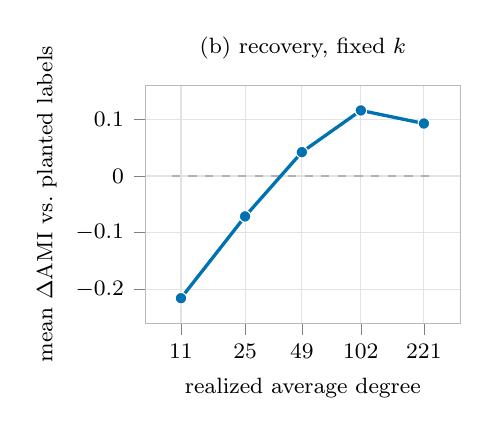
\begin{tikzpicture}
\begin{axis}[
    width=0.46\textwidth, height=4.6cm,
    xmode=log, log basis x=10,
    xlabel={realized average degree},
    ylabel={mean $\Delta\mathrm{AMI}$ vs.\ planted labels},
    xtick={11.2,24.6,49.4,101.9,220.9},
    xticklabels={11,25,49,102,221},
    xticklabel style={font=\footnotesize},
    scaled y ticks=false,
    yticklabel style={font=\footnotesize,
                      /pgf/number format/fixed,
                      /pgf/number format/precision=2},
    xlabel style={font=\footnotesize},
    ylabel style={font=\footnotesize},
    title={\footnotesize (b) recovery, fixed $k$},
    ymin=-0.26, ymax=0.16,
    tick align=outside, tick pos=left,
    axis line style={gray!55},
    grid=major, major grid style={gray!22}]
  \addplot[gray!60, dashed, line width=0.6pt, forget plot, mark=none]
      coordinates {(10,0) (250,0)};
  \addplot[cbblue, line width=1.2pt, mark=*, mark size=2.1pt,
           mark options={fill=cbblue, draw=white, line width=0.4pt}]
      coordinates {(11.2,-0.2160) (24.6,-0.0715) (49.4,0.0421)
                   (101.9,0.1158) (220.9,0.0927)};
\end{axis}
\end{tikzpicture}
\caption{Where the two regimes separate, L-Spar on LFR graphs at realized mixing
near $0.6$, means over twelve configurations per degree. Panel (a) is the mean
$\Delta Q$ column of Table~\ref{tab:boundary} together with the same quantity for
a free-granularity optimizer on the identical graphs, measured against the best
of five plain restarts. The fixed-$k$ arm crosses zero between average degree
$49$ and $102$; the free-granularity arm does not reach $+0.005$ at any degree,
which is what makes the boundary a boundary rather than a threshold in density
alone. Panel (b) is the mean $\Delta\mathrm{AMI}$ column of the same table, and
recovery crosses at a lower density than the objective does. The
free-granularity arm's recovery comparison uses a different baseline, the
resolution-matched partition of the untouched graph, and is given in the text
rather than plotted here.}
\label{fig:boundary}
\end{figure*}
